% Capítulo 6. Estrategia de solución e implementación (rúbrica estrategia 15 pts e implementación 5 pts).

Como el modelo del capítulo~\ref{ch:modelo} no se puede resolver para la red completa, el plan se obtiene con un método híbrido que arma una solución factible y luego la mejora por partes. La Figura~\ref{fig:flujo} muestra el procedimiento completo, sin detalles de código, y las secciones siguientes explican cada paso.

\begin{figure}[htbp]
\centering
\begin{tikzpicture}[node distance=14mm and 5mm,
  caja/.style={draw, rounded corners, align=center, font=\footnotesize, minimum height=11mm, text width=25mm},
  dato/.style={caja, fill=black!5}, flecha/.style={-Stealth}]
\node[dato] (dat) {Corridas, distancias\\ y parámetros};
\node[caja, right=of dat] (sec) {Sectores\\{\scriptsize cada ruta a su\\ electroterminal}};
\node[caja, right=of sec] (ini) {Plan inicial\\{\scriptsize corridas en orden\\ de salida}};
\node[caja, right=of ini] (sor) {Sorteo de\\ cuatro buses\\{\scriptsize del mismo sector}};
\node[caja, below=of sor] (mov) {Propuestas\\{\scriptsize absorción\\ y rotación}};
\node[caja, left=of mov] (milp) {MILP local\\{\scriptsize terminales y recargas\\ de las cuatro\\ jornadas}};
\node[caja, left=of milp] (aud) {Auditor\\{\scriptsize se acepta si es\\ factible y más barato}};
\node[dato, left=of aud] (sal) {Plan final\\{\scriptsize jornada de cada bus\\ e indicadores}};
\draw[flecha] (dat) -- (sec);
\draw[flecha] (sec) -- (ini);
\draw[flecha] (ini) -- (sor);
\draw[flecha] (sor) -- (mov);
\draw[flecha] (mov) -- (milp);
\draw[flecha] (milp) -- (aud);
\draw[flecha, dashed] (aud.north) to[out=80, in=200] node[pos=.55, fill=white, font=\scriptsize, inner sep=1pt]{se repite hasta agotar el tiempo} (sor.south west);
\draw[flecha] (aud) -- (sal);
\end{tikzpicture}
\caption{Procedimiento del método híbrido. La búsqueda repite el sorteo, las propuestas, el MILP local y la auditoría hasta agotar su tiempo, y el plan que sale siempre es factible.}
\label{fig:flujo}
\end{figure}

\section{Sectores y plan inicial}
\label{sec:construccion}

El primer paso asocia cada ruta a un electroterminal, como se describió en la sección~\ref{sec:energia-datos}. Cada bus atiende corridas de un solo sector, aunque puede cargar en cualquier electroterminal.

El plan inicial se arma recorriendo las corridas en orden de hora de salida. Para cada una se revisan los buses del sector que ya están en servicio y se descartan los que no alcanzan a llegar a tiempo a su origen o no tienen energía suficiente para el traslado, la corrida y un regreso de respaldo a un terminal sin bajar de la reserva. Entre los que quedan se elige el de menor traslado en vacío. Si a un bus le falta energía, se intenta intercalar una visita a un electroterminal en el hueco previo, cargando solo lo necesario y verificando que haya plaza y conexión durante toda la visita. Si ningún bus puede tomar la corrida, se agrega uno nuevo, con la batería llena, desde el terminal común más cercano. Este paso no usa optimización y toma \SegundosInicial~segundos para el día laboral completo.

Frente al caso base, el plan inicial ya cambia tres cosas. Comparte buses entre todas las rutas del sector, carga solo la energía que falta en vez de llenar la batería, y elige el bus que queda más cerca. Con eso logra \BusesInicialLaboral{} buses en día laboral, y explica el \PctAhorroInicial\,\% de la reducción total de flota (sección~\ref{sec:origen-ahorro}).

\section{Mejora por grupos de buses}
\label{sec:mejora}

La mejora toma grupos de cuatro jornadas del mismo sector y busca una forma más barata de repartir sus corridas. Los cuatro buses se sortean con una semilla fija, lo que permite repetir exactamente una corrida del método. Dentro del grupo se prueban dos operaciones, que muestra la Figura~\ref{fig:operaciones}.

\begin{figure}[htbp]
\centering
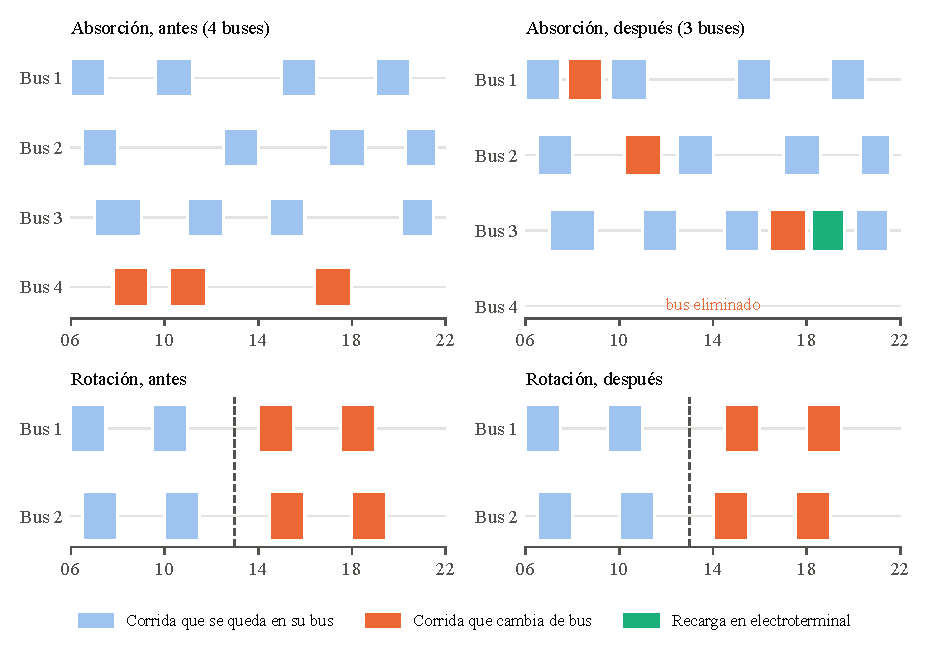
\includegraphics[width=\textwidth]{figures/operaciones.pdf}
\caption{Las dos operaciones de la mejora, con horarios ilustrativos. En la absorción, el bus con menos corridas las reparte entre los otros tres y, si al bus 3 ya no le alcanza la batería, el MILP local le agrega una recarga. En la rotación, dos buses intercambian todo lo que hacen después de un corte (línea punteada).}
\label{fig:operaciones}
\end{figure}

En la absorción, el bus que menos corridas tiene intenta repartirlas entre los otros tres. Cada corrida se inserta en un hueco compatible de algún receptor, y como hay muchas formas de hacerlo se conservan solo unas pocas alternativas parciales, ordenadas por kilómetros en vacío y por lo pareja que queda la carga de trabajo. Si todas las corridas encuentran lugar, el grupo pasa de cuatro buses a tres, y el plan ahorra USD~\CostoBus{} diarios más lo que cambien los kilómetros y la energía. En la rotación, cada jornada se corta en un punto y las partes finales se intercambian entre los buses, sin tocar los comienzos. La rotación no elimina buses, pero puede acortar traslados o dejar espacio para una absorción posterior.

\section{El MILP local y la aceptación}
\label{sec:milp-local}

Cada propuesta define qué corridas hace cada bus y en qué orden, pero todavía no dice si los buses tienen energía para hacerlas ni dónde cargan. Ese es el papel del MILP local. Con las corridas de cada jornada ya fijas, decide en qué terminal parte cada bus, si recarga en cada hueco, en qué electroterminal y cuánto, y dónde termina el día. Lo hace minimizando los kilómetros en vacío, las sesiones y el costo de la energía, y respetando el balance de energía, la reserva, la capacidad de la batería, la potencia de carga y la capacidad que dejan libre en cada electroterminal los buses que no están en el grupo. Es el modelo del capítulo~\ref{ch:modelo} con el orden de las corridas fijo y restringido a cuatro jornadas, y su formulación completa está en el anexo~\ref{an:milp-local}.

Se resuelve con Gurobi, con un límite de dos segundos por intento, una tolerancia de 2\,\% y un hilo. Si no encuentra solución factible, la propuesta se descarta. Si la encuentra, el plan candidato se reconstruye y el auditor lo revisa completo. El cambio se acepta solo si el auditor lo aprueba y el costo total baja. Por eso la búsqueda nunca empeora el plan y puede detenerse en cualquier momento con un plan factible. En la corrida final del día laboral, cada semilla probó en promedio \IntentosCuartetos{} propuestas en \MinutosFinal{} minutos y aceptó \MejorasCuartetos.

\section{Por qué cuatro buses elegidos al azar}
\label{sec:por-que-cuartetos}

El tamaño del grupo es el dilema que describen \citeA{ahuja_vlsn_2002}. Un grupo más grande ofrece más formas de repartir las corridas, pero cada propuesta tarda más en resolverse y en el mismo tiempo se prueban menos. Para elegirlo se compararon grupos de 2 a 8 buses, elegidos al azar o por tener horarios parecidos, todos con el mismo tiempo y en el mismo computador, en la red completa y en casos chicos con óptimo conocido. La regla acordada por el grupo fue quedarse con el método más barato a igual tiempo. Ganó el grupo de cuatro buses elegidos al azar, y los detalles están en la sección~\ref{sec:metodo-elegido}.

\section{Validación con el modelo exacto}
\label{sec:validacion}

Para medir la calidad del método se resolvió el modelo del capítulo~\ref{ch:modelo} al óptimo en casos chicos, de 2 a 4 rutas de un mismo sector, y en casos medianos de 6 a 12 rutas con la versión podada. Los casos usan las mismas corridas, distancias, costos y reglas que la red completa, así que el óptimo es una vara directa. Además, como con la batería de \Bateria~kWh casi ningún bus necesita recargar en esos casos, se crearon copias con baterías de 150 y 120~kWh para obligar a recargar y probar el método donde la carga sí pesa. Con 100~kWh ya no hay solución, porque algunas corridas, contando el traslado de salida y el de regreso, necesitan entre 105 y 112~kWh.

\section{Implementación y herramientas}
\label{sec:implementacion}

Todo está escrito en Python. Los modelos enteros se resuelven con Gurobi~12 a través de \texttt{gurobipy}, con licencia académica, porque la licencia gratuita que trae el paquete solo admite modelos de hasta dos mil variables y no alcanza para grupos de tres buses o más. El método está en la carpeta \texttt{metodo\_hibrido} del repositorio, el caso base en \texttt{codigo/tres\_fases} y los estudios de la Entrega~3 en \texttt{09-entrega3}. Todo se corrió en un mismo computador (Mac M1 con 8~GB de memoria), porque la búsqueda se corta por reloj y depende del equipo.

El auditor (\texttt{verificar.py}) es independiente del constructor y de la búsqueda. Reconstruye cada plan desde sus actividades y comprueba que cada corrida se cubra una vez con su horario, que cada bus llegue a tiempo a su siguiente actividad, que ninguna jornada cruce sectores, que la energía no baje de la reserva, que no se excedan plazas ni conexiones y que el costo informado coincida con el recalculado. Ningún plan de este informe se usó sin pasar por él, incluidos los del caso base y los del modelo exacto.

Cada corrida guarda sus parámetros, las versiones del software y una huella SHA-256 de cada archivo de entrada y de código. Un script genera todas las cifras del informe desde los resultados, y el anexo~\ref{an:reproduccion} indica cómo repetir cada una.
